\chapter{Results}
\label{ch:results}

[brief introduction of the chapter]

% \section{Smart Contract Interactions}
% \label{sec:smart_contract_interactions}

Like mentioned, the blockchain is a public ledger that stores all the
transactions that are made, so we can see all the interactions with the smart
contracts. We deployed the smart contracts on a testnet, so that we don't have
to use real funds. This way we can simulate what would happen on the mainnet
without any risks or cost. This was done with Foundry, like mentioned before,
and we created some scripts to populate the system to be able to see it on the
blockchain. These scripts deploy the smart contracts, adds an organizer,
creates a few events, and adds some packages to each.

For each network there is an explorer that allows us to see all the
transactions that are made, and the Figure \ref{fig:ticketchain_transactions}
shows what it looks like.
\begin{figure}[H]
    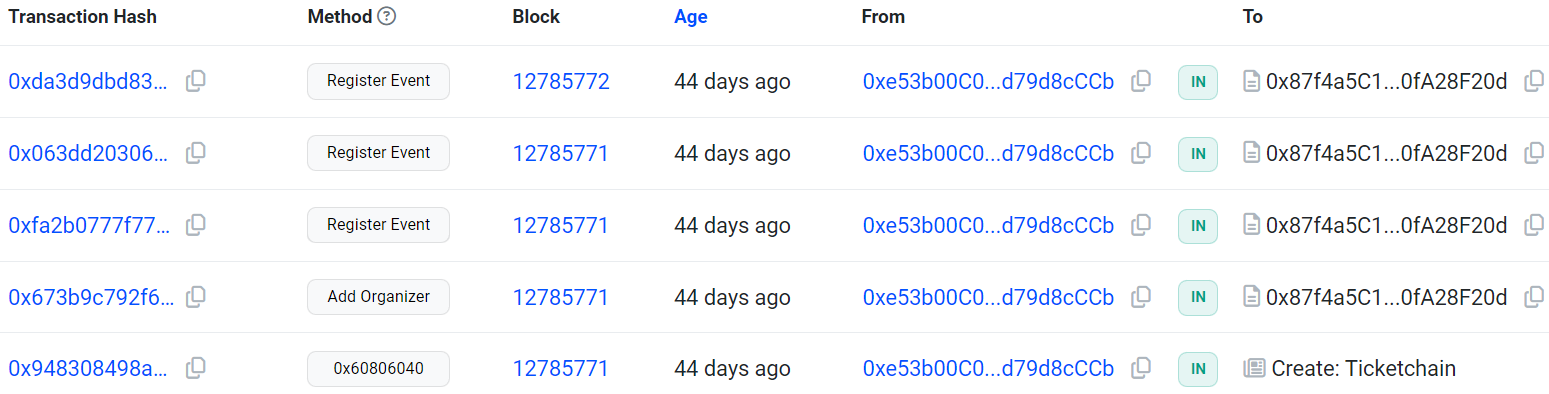
\includegraphics[width=\textwidth]{Ticketchain transactions.png}
    \centering
    \caption{Ticketchain transactions}
    \label{fig:ticketchain_transactions}
\end{figure}

We can see when the contract was deployed, the adding of an organizer to the
system, and the creation of 3 events. This information is what's then loaded in
the app, as was previously shown in the Figure \ref{fig:home_page}.

\section{Buy Tickets}
\label{sec:buy_tickets}

For the user to buy tickets, he will have to proceed the way mentioned in the
Section \ref{subsec:events}. The previous Figures \ref{fig:home_page} and
\ref{fig:tickets_page} show that we only have tickets for 2 events while there
are 3 available, so we're going to show the process of buying tickets for the
third one. Looking into the event page, we see there is only one package
available with 100 tickets, like the Figure \ref{fig:buy_tickets_event} shows.

\begin{figure}[H]
    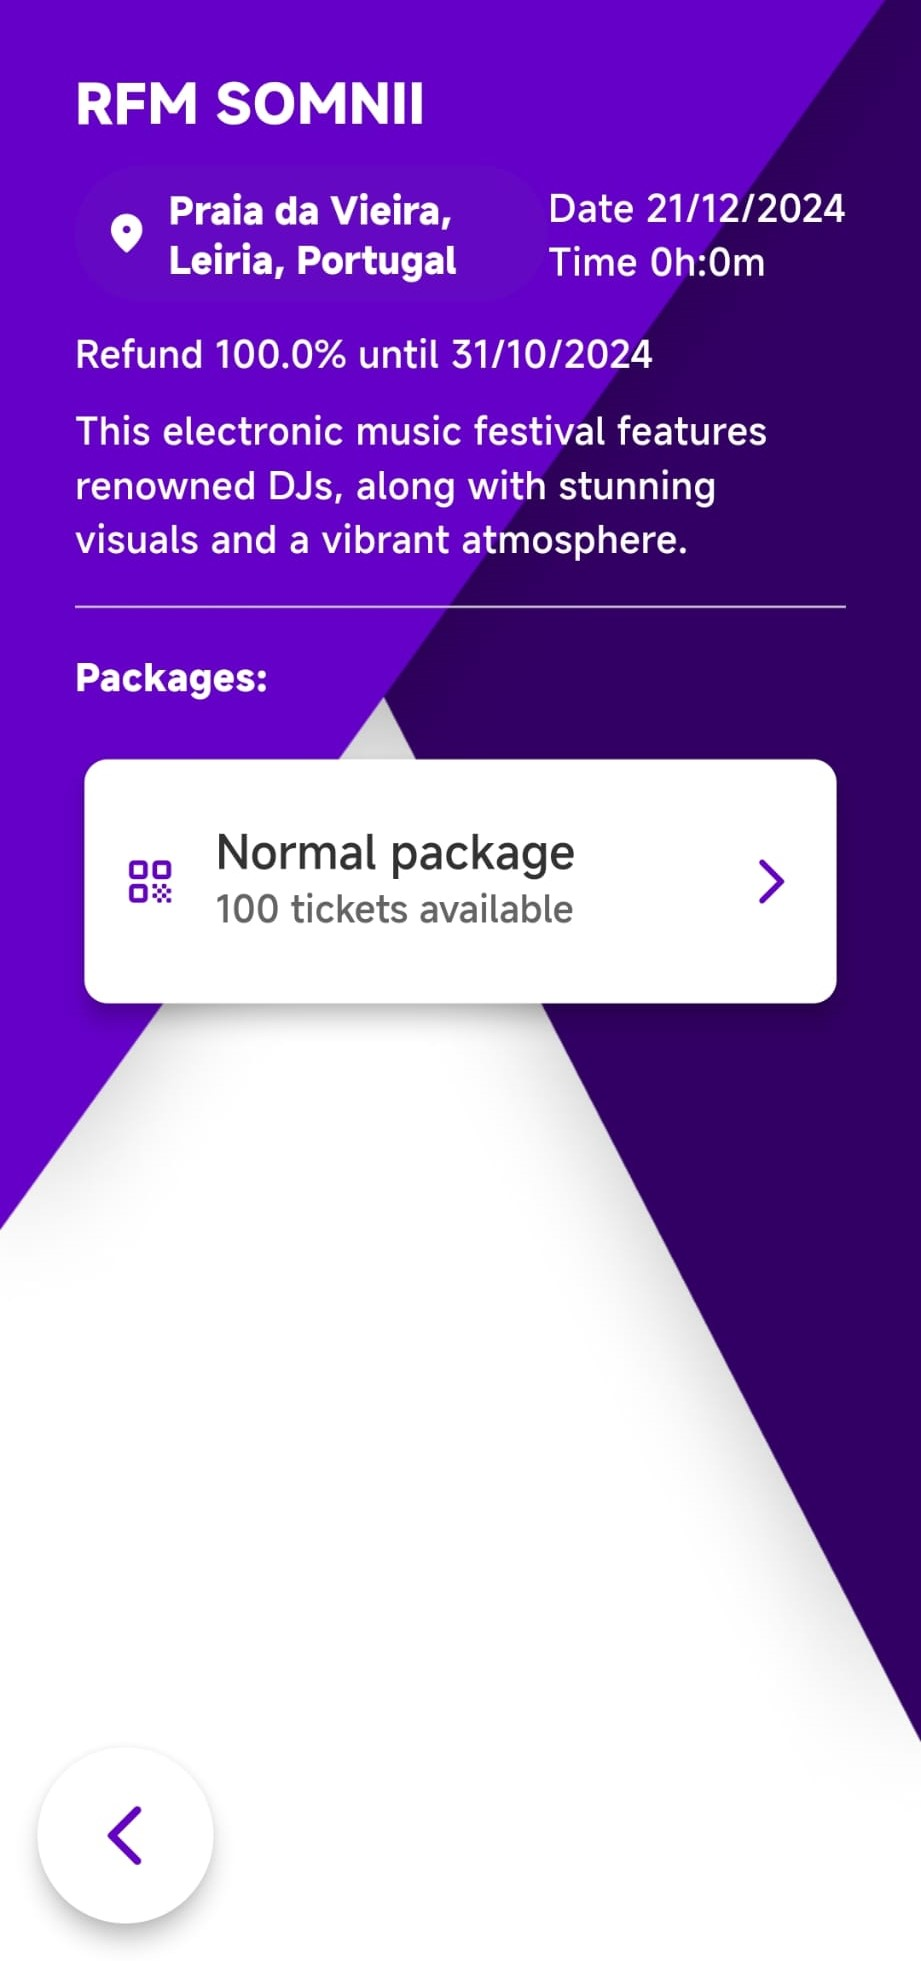
\includegraphics[width=\textwidth/3,frame]{Event page 2.jpg}
    \centering
    \caption{Third event page}
    \label{fig:buy_tickets_event}
\end{figure}

When we click on the package, we see the prompt to buy tickets, and like we see
in the Figure \ref{fig:buy_tickets_prompt}, we're going to buy 3 tickets.

\begin{figure}[H]
    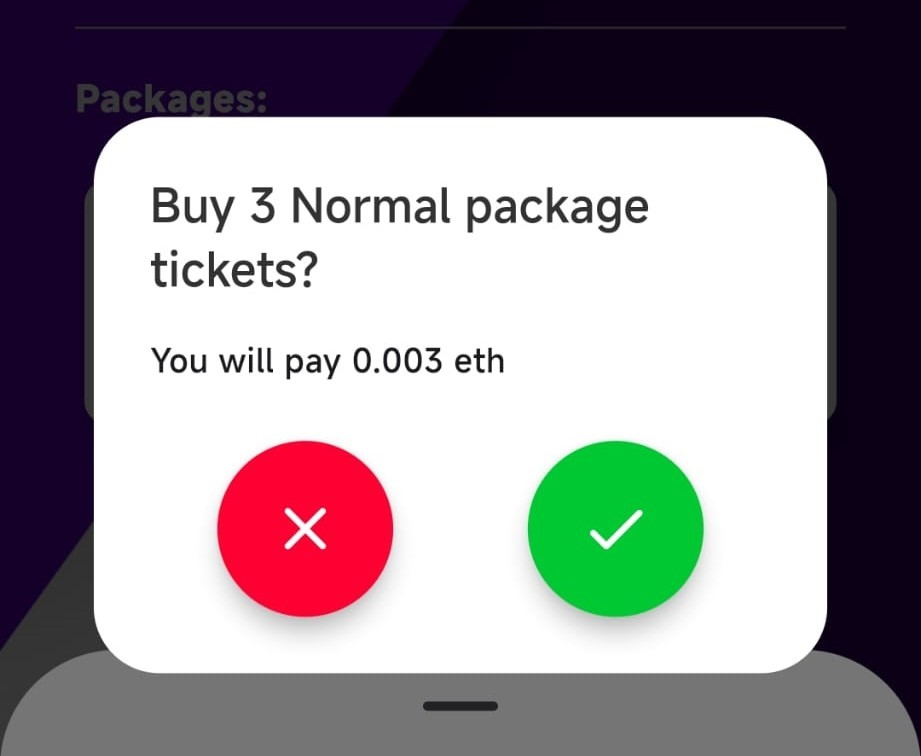
\includegraphics[width=\textwidth/3,frame]{Buy tickets prompt 2.jpg}
    \centering
    \caption{Buy 3 tickets prompt}
    \label{fig:buy_tickets_prompt}
\end{figure}

After confirming the prompt, the wallet opens and we see the transaction to be
approved, as shown in the Figure \ref{fig:buy_tickets_transaction}.

\begin{figure}[H]
    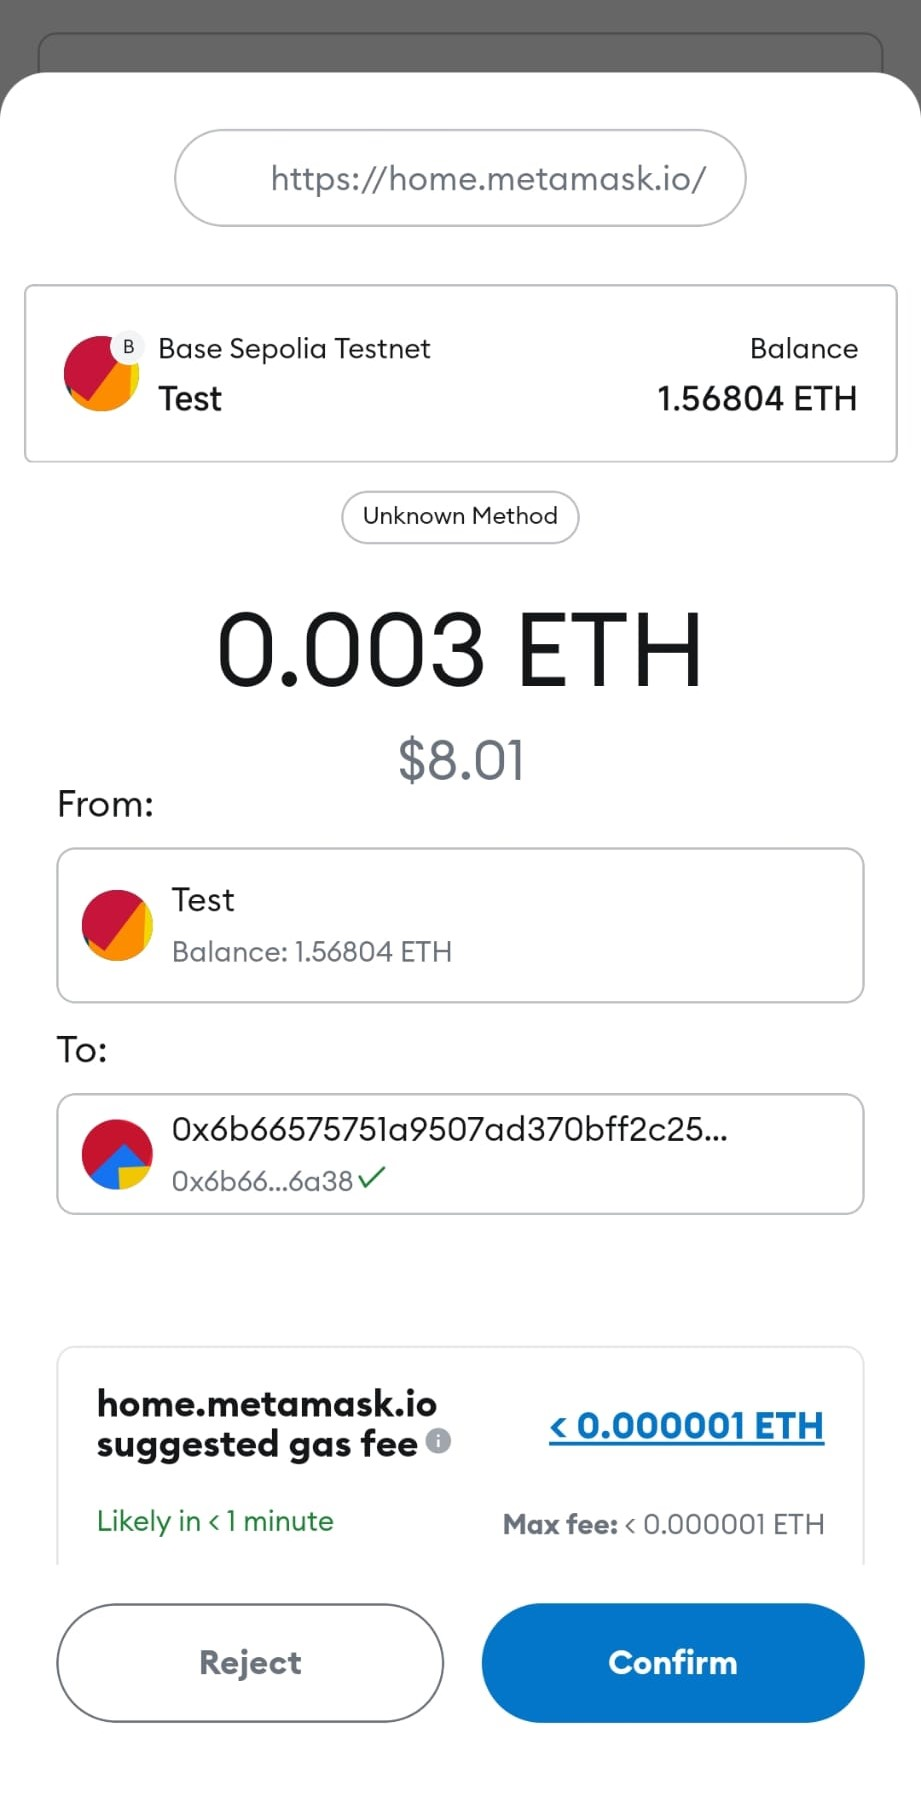
\includegraphics[width=\textwidth/3,frame]{MetaMask transaction prompt 2.jpg}
    \centering
    \caption{Buy 3 tickets transaction}
    \label{fig:buy_tickets_transaction}
\end{figure}

We can see that we're sending 0.003 eth in the transaction to buy the tickets.
After confirmation, we see the tickets being successfully purchased, and we see
the update on the profile page, in the Figure \ref{fig:profile_page_2}, which
as now the third event with 3 tickets.

\begin{figure}[H]
    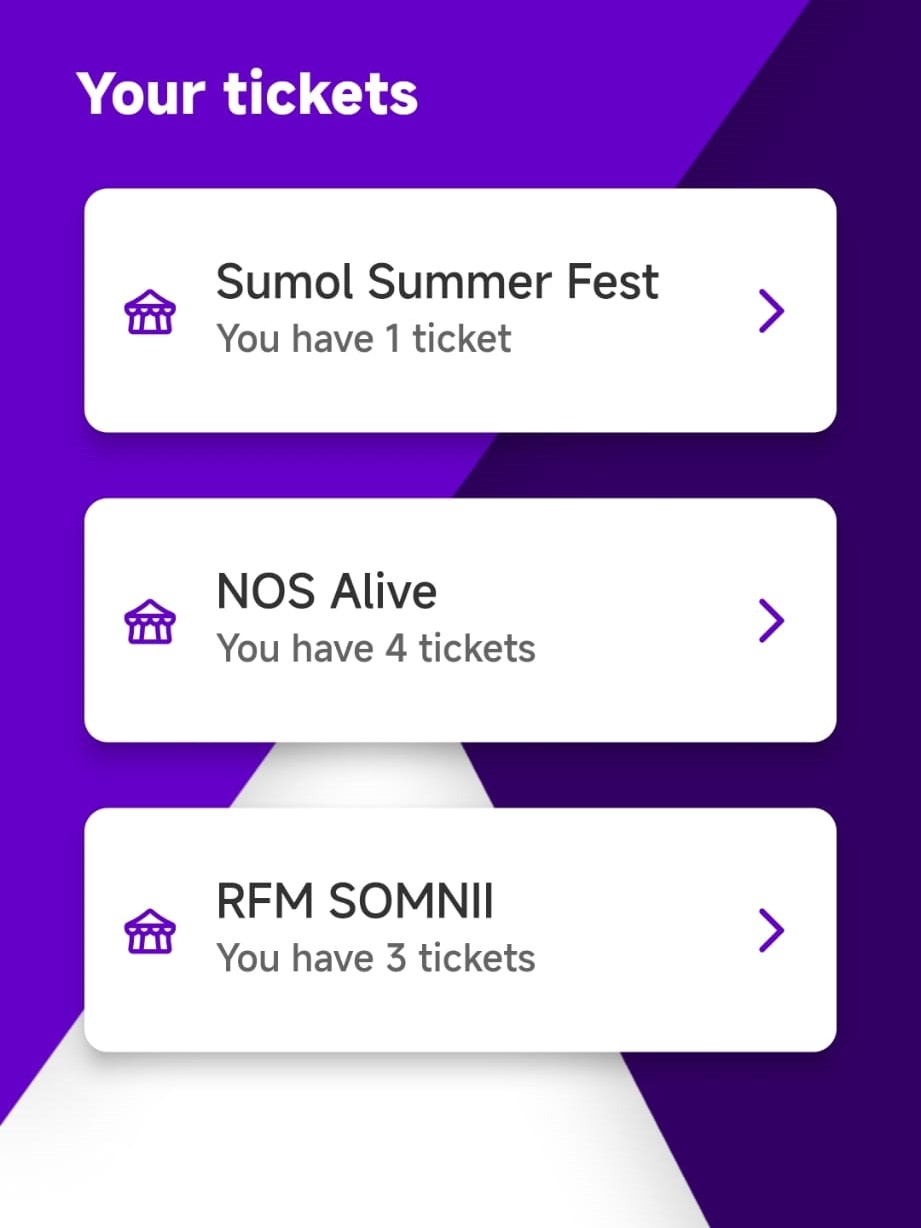
\includegraphics[width=\textwidth/3,frame]{Profile page 2.jpg}
    \centering
    \caption{Profile page with the third event}
    \label{fig:profile_page_2}
\end{figure}

Going back to the event page we see now that there are only 97 tickets left,
like the Figure \ref{fig:buy_tickets_event_2} shows.

\begin{figure}[H]
    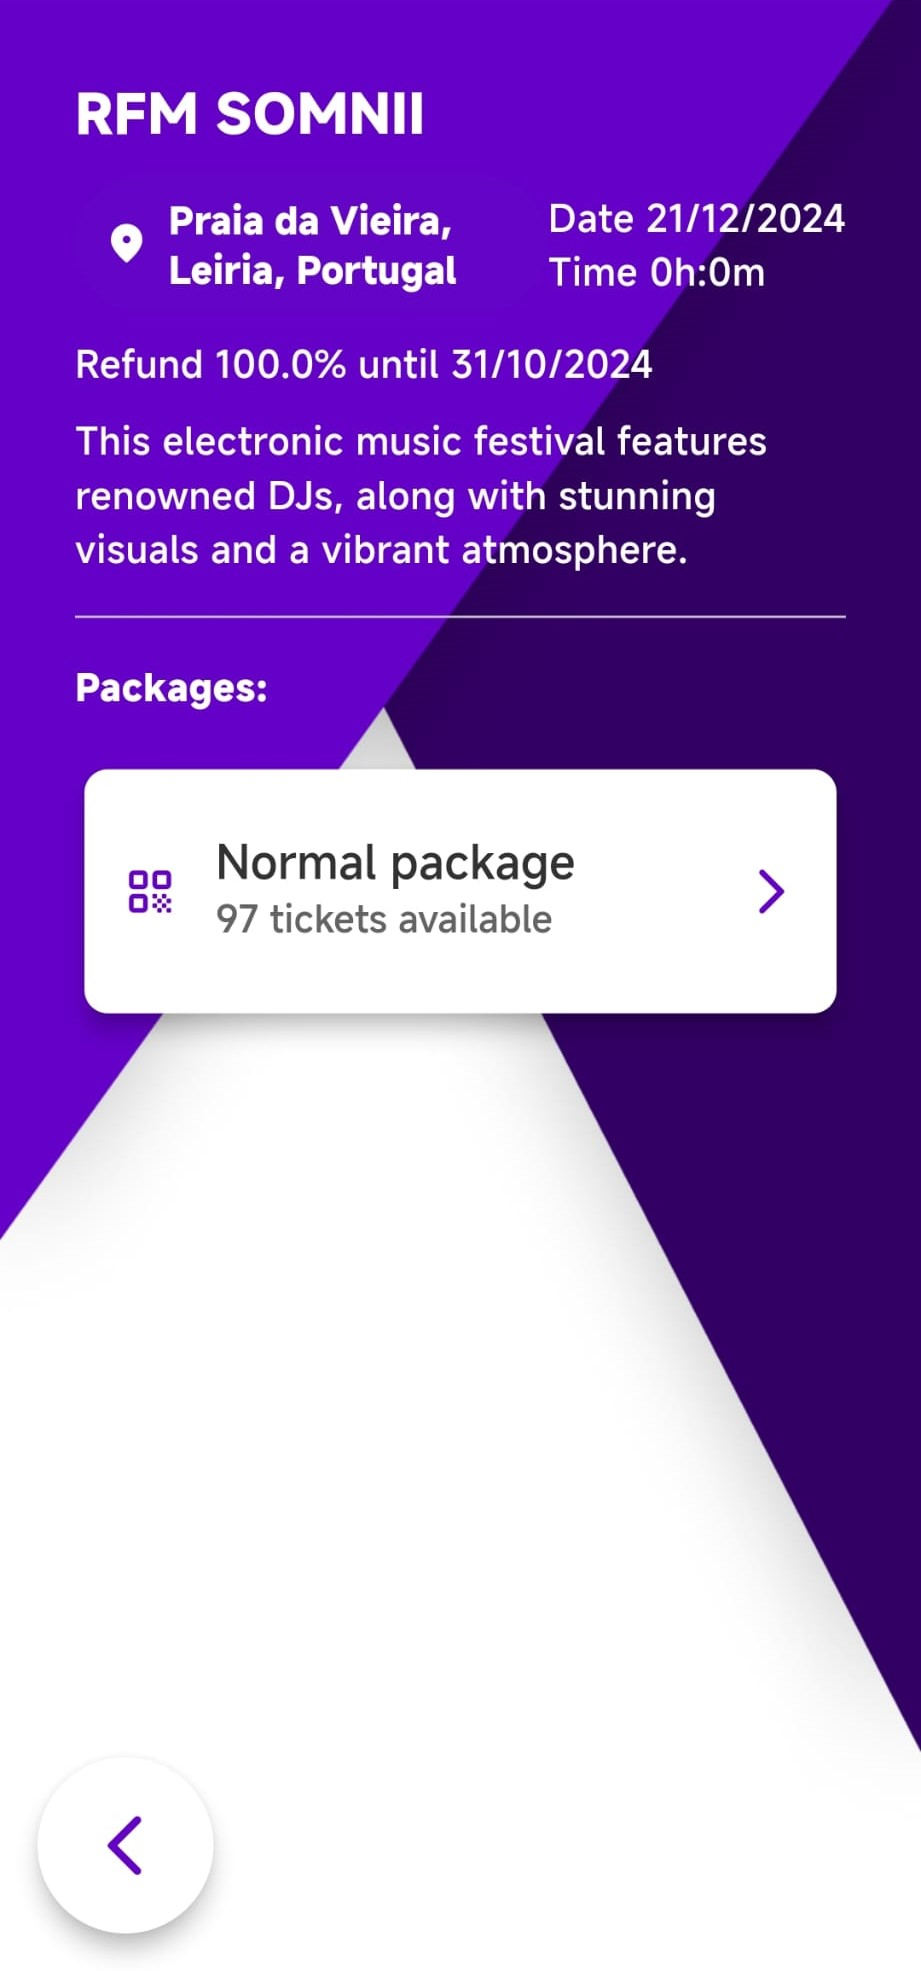
\includegraphics[width=\textwidth/3,frame]{Event page 3.jpg}
    \centering
    \caption{Third event page with 97 tickets}
    \label{fig:buy_tickets_event_2}
\end{figure}

Going to the blockchain explorer to see the registered transaction, we can
search for our address and we see that there is a recent \textit{Buy Tickets}
transaction, like the Figure \ref{fig:user_transactions} shows.

\begin{figure}[H]
    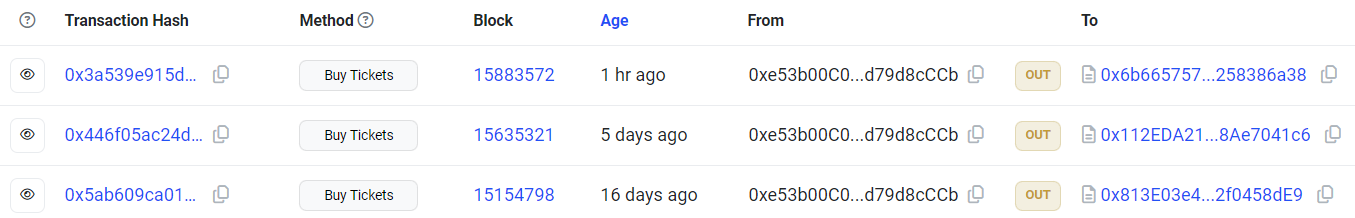
\includegraphics[width=\textwidth]{User transactions.png}
    \centering
    \caption{User transaction}
    \label{fig:user_transactions}
\end{figure}

The \textit{To} column shows the address who was interacted with and the
\textit{Transaction Hash} column shows the unique identifier of the
transaction. Taping the transaction hash, we will be sent to a page where we
see the details of the transaction, like the Figure
\ref{fig:buy_tickets_transaction_details} shows.

\begin{figure}[H]
    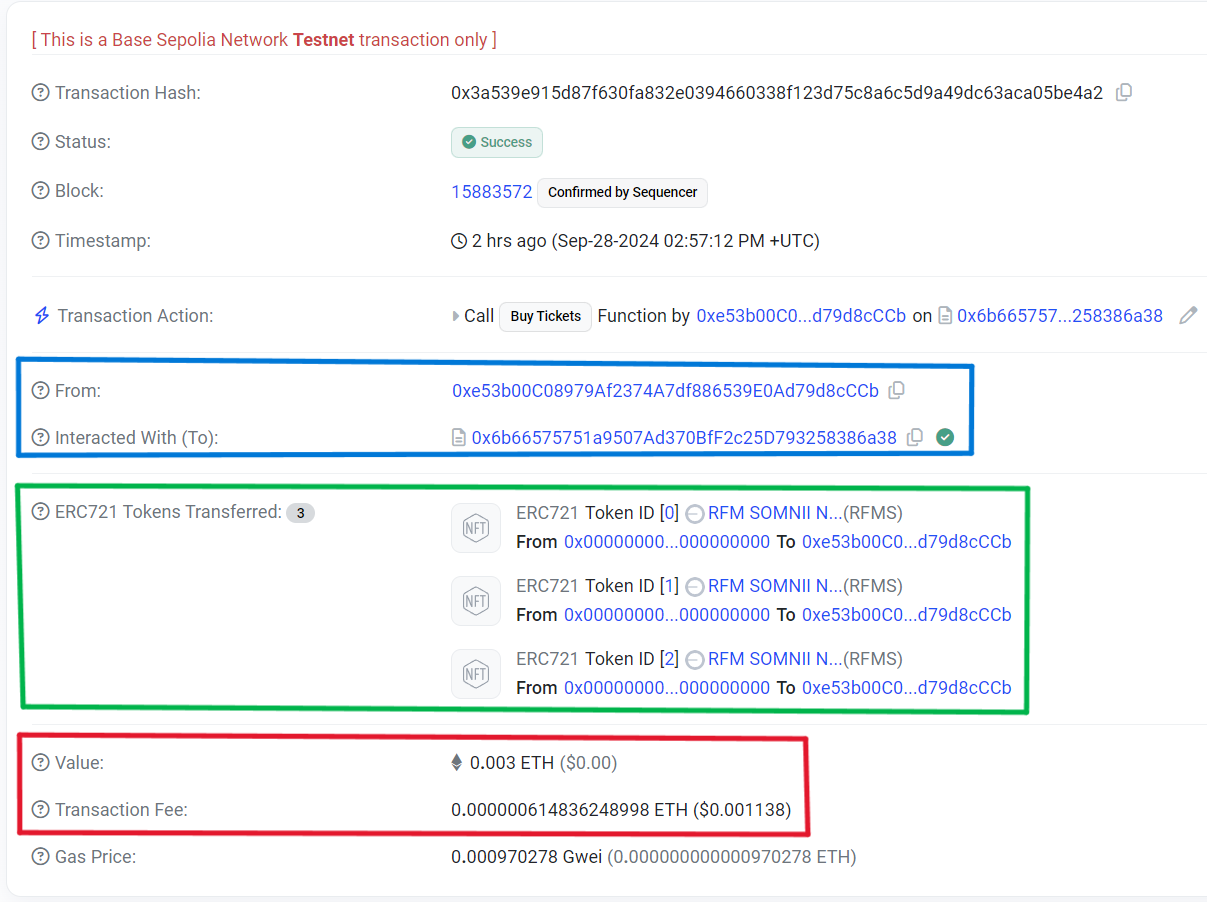
\includegraphics[width=\textwidth]{Buy tickets transaction details.png}
    \centering
    \caption{Buy tickets transaction details}
    \label{fig:buy_tickets_transaction_details}
\end{figure}

The main takeaways from here are the boxes highlighted. The one in blue shows
the addresses of who interacted with whom. In this case the \textit{From} is
our user address, and the \textit{To} is the event address.

The one in green shows the NFTs that were transferred. The explorer detects
these NFTs because it sees that the contract is extending the ERC721 standard,
so it displays in a more readable way. We can see we that the NFTs with IDs 0,
1, and 2 were transferred to our address, which came from the \textit{null}
address (0x00\dots00), meaning that they were minted.

The one in red shows the value that was sent in the transaction, which is the
total price of the tickets, 0.003 eth, and also the network fee that was paid
for the transaction.

\section{Gift Tickets}
\label{sec:gift_tickets}

For the process of gifting tickets, we used another wallet just to check if the
app updates accordingly. The Figure \ref{fig:gift_tickets_prompt} shows the
prompt when the user is going to gift the tickets.

\begin{figure}[H]
    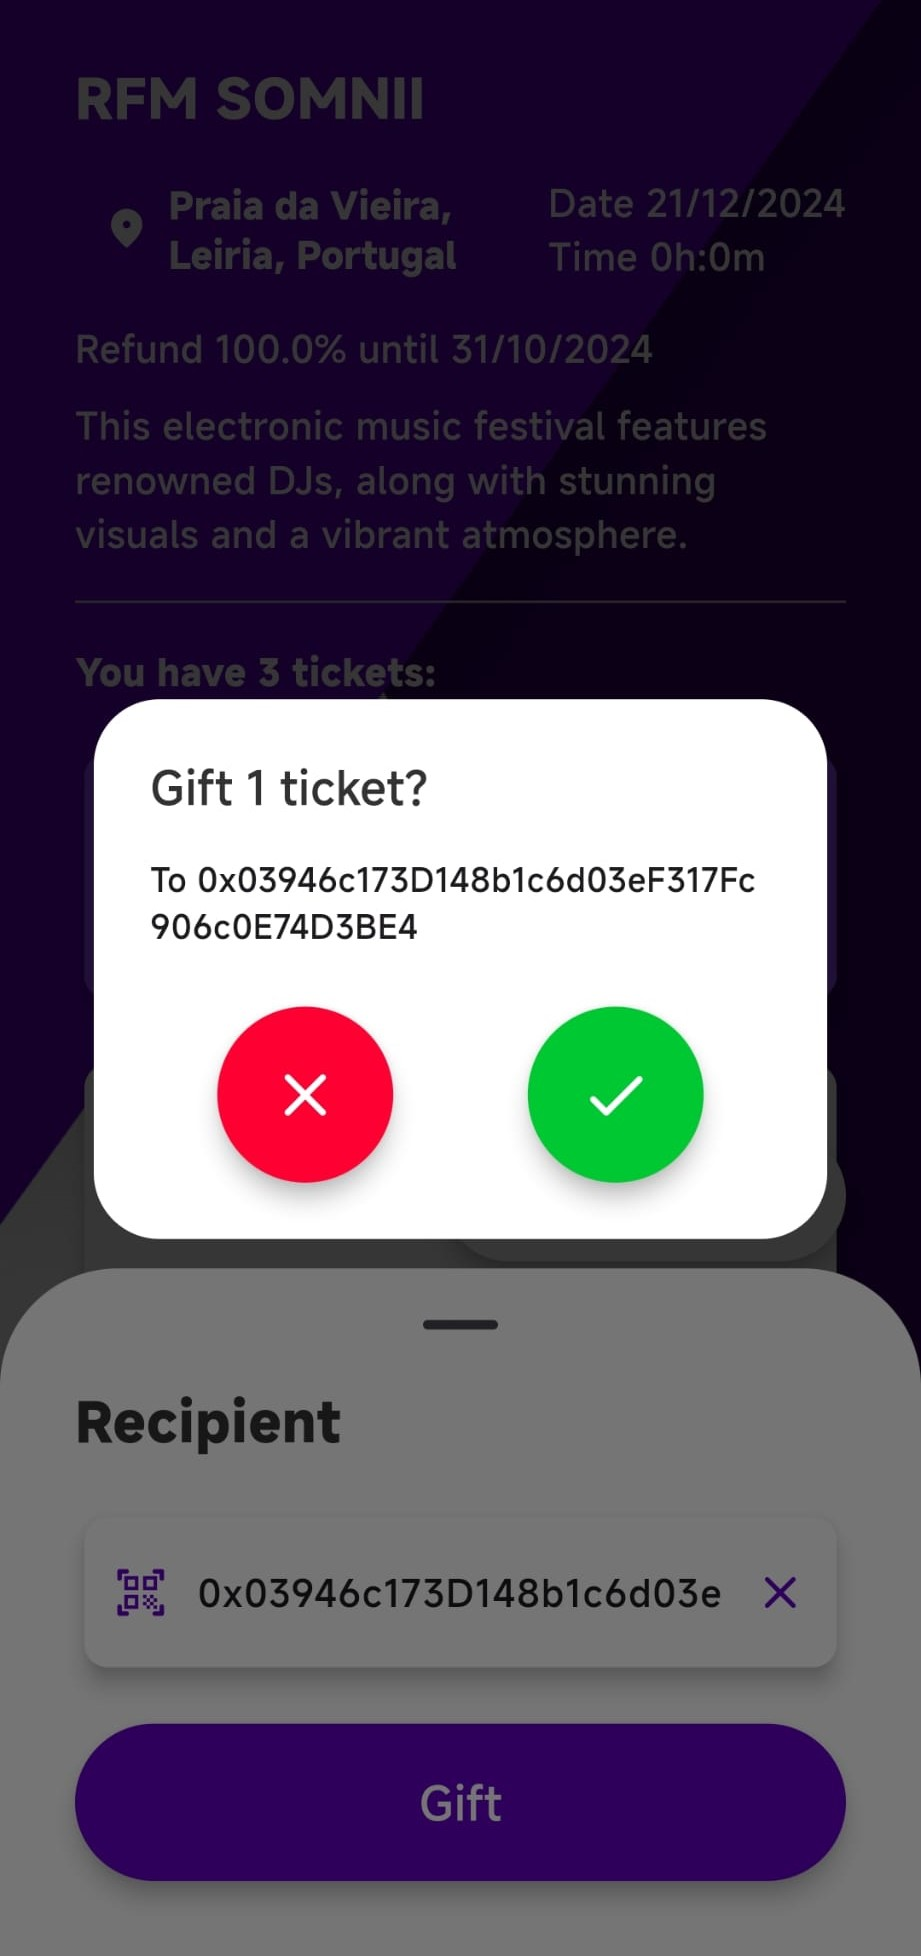
\includegraphics[width=\textwidth/3,frame]{Gift tickets prompt.jpg}
    \centering
    \caption{Gift tickets prompt}
    \label{fig:gift_tickets_prompt}
\end{figure}

After executing the transaction, we logged out of the app and authenticated
with the other address to check that the ticket appears on the profile page of
that user. The Figure \ref{fig:profile_page_3} shows the profile page of the
user that received the tickets and we can confirm that the transfer was
successful.

\begin{figure}[H]
    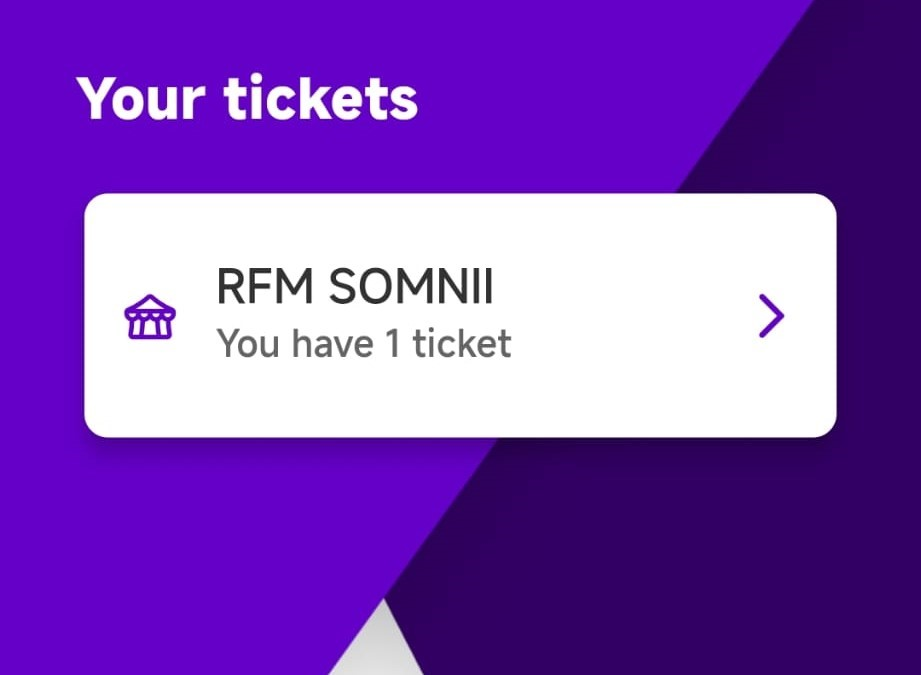
\includegraphics[width=\textwidth/3,frame]{Profile page 3.jpg}
    \centering
    \caption{Profile page with the gifted ticket}
    \label{fig:profile_page_3}
\end{figure}

The blockchain explorer shows the transaction of the gift operation, and the
Figure \ref{fig:gift_tickets_transaction_details} shows the details of it.

\begin{figure}[H]
    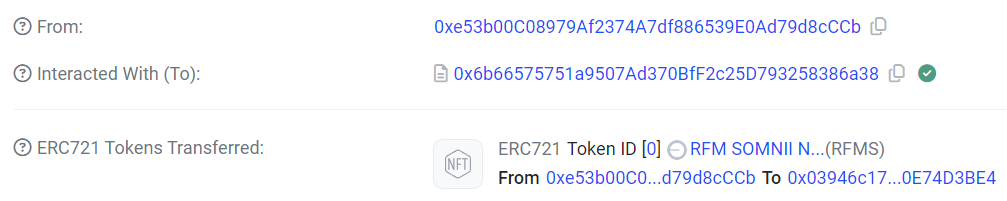
\includegraphics[width=\textwidth]{Gift tickets transaction details.png}
    \centering
    \caption{Gift tickets transaction details}
    \label{fig:gift_tickets_transaction_details}
\end{figure}

We see above the interaction between our user address (0xe5{\dots}Cb) and the
address of the event (0x6b\dots38), and on the NFT operation below we see that
the NFT with ID 0 went from our address (0xe5{\dots}Cb) to the address of our
other user (0x03{\dots}E4).

\section{Refund Tickets}
\label{sec:refund_tickets}

The process of refunding tickets is similar to the process of gifting them, but
in this case the user will \textit{burn} the tickets in exchange for the
refund. The Figure \ref{fig:refund_tickets_prompt} shows the prompt that shows
the user the amount he's going to receive, which in the case of this event is
100\%. Note that we paid 0.003 eth for the 3 tickets.

\begin{figure}[H]
    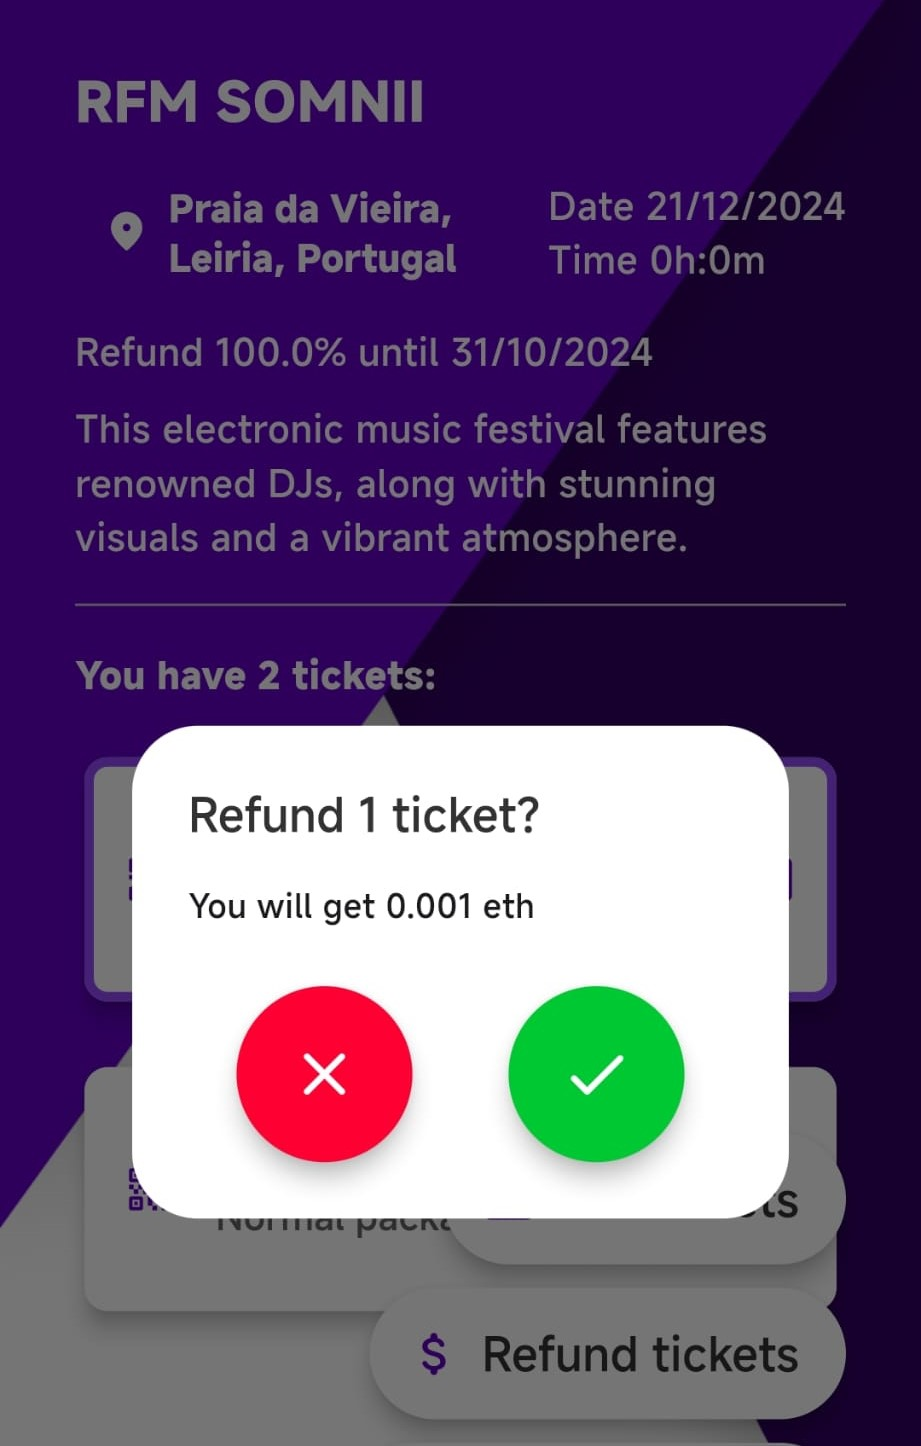
\includegraphics[width=\textwidth/3,frame]{Refund tickets prompt.jpg}
    \centering
    \caption{Refund tickets prompt}
    \label{fig:refund_tickets_prompt}
\end{figure}

After executing the transaction, we see the refund being made, and the Figure
\ref{fig:refund_tickets_transaction_details} shows the details of it.

\begin{figure}[H]
    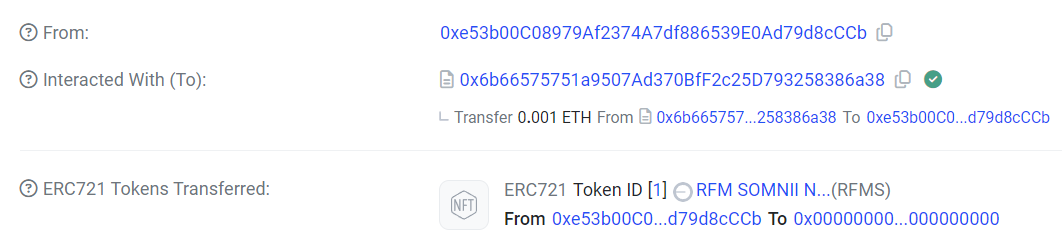
\includegraphics[width=\textwidth]{Refund tickets transaction details.png}
    \centering
    \caption{Refund tickets transaction details}
    \label{fig:refund_tickets_transaction_details}
\end{figure}

Once again, we see our user address (0xe5{\dots}Cb) interacting the address of
the event (0x6b\dots38), and sending our NFT with the ID 1 to the \textit{null}
address (0x00\dots00), meaning that they were burned, becoming again available
for purchase. We can confirm that we got the refund because on the entry above
we also see the transfer of 0.001 eth from the contract's address (0x6b\dots38)
to our user address (0xe5{\dots}Cb).

To show that the tickets are available again, we see in the event page that the
package that had 97 tickets left, has now 98, like the Figure
\ref{fig:refund_tickets_event} shows.

\begin{figure}[H]
    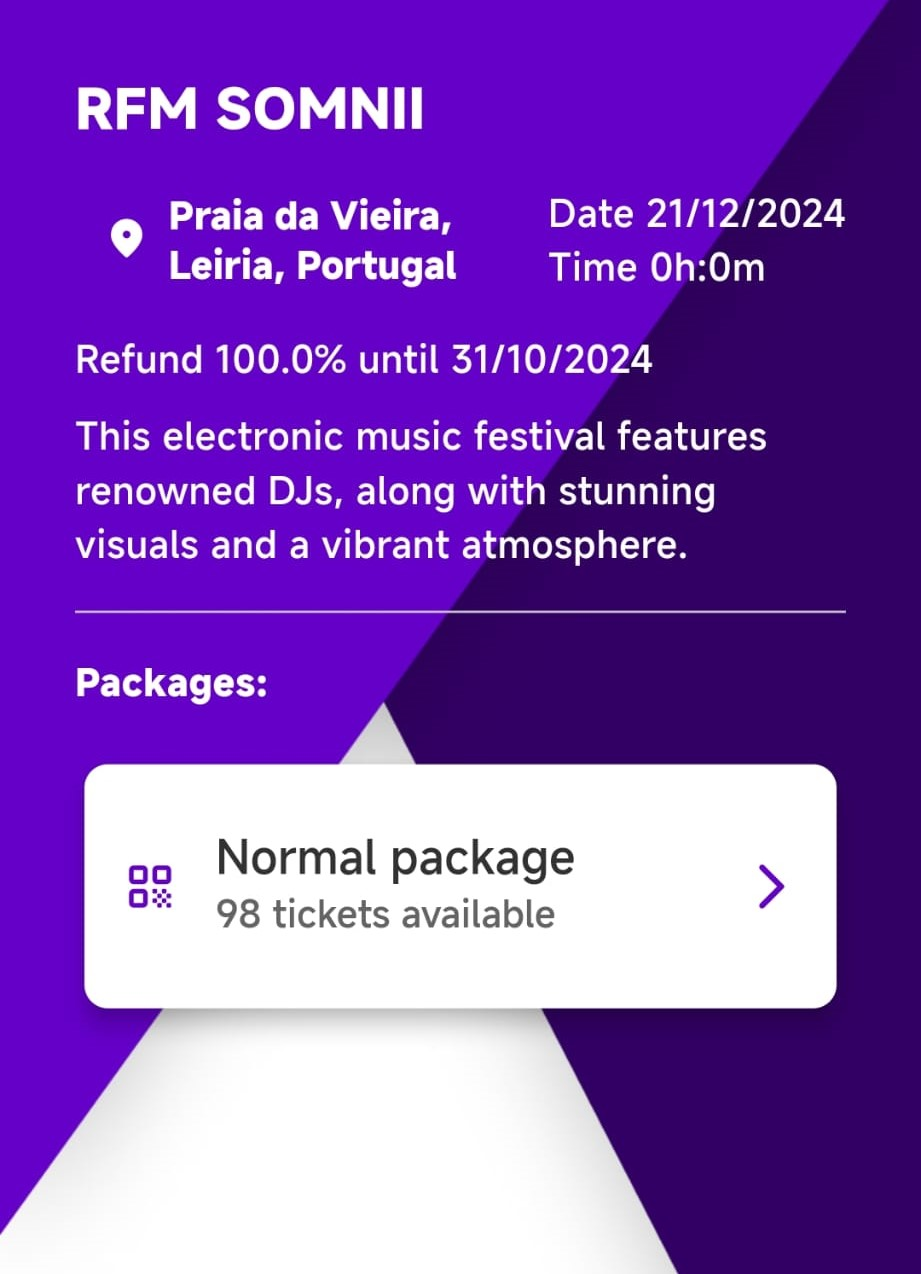
\includegraphics[width=\textwidth/3,frame]{Event page 4.jpg}
    \centering
    \caption{Third event page with 98 tickets}
    \label{fig:refund_tickets_event}
\end{figure}

\section{Validate Tickets}
\label{sec:validate_tickets}
